\documentclass[11pt]{article}

\usepackage{physics}
\usepackage[top=1in, bottom=1in, left=0.5in, right=0.5in]{geometry}
\usepackage{hanging}
\usepackage{amsfonts, amsmath, amssymb}
\usepackage[none]{hyphenat}
\usepackage{fancyhdr}
\usepackage[nottoc, notlot, notlof]{tocbibind}
\usepackage{graphicx}
\graphicspath{{./images/}}
\usepackage{float}
\usepackage{siunitx}
\usepackage{esint}

\pagestyle{fancy}
\fancyhead{}
\fancyfoot{}
\fancyhead[L]{MAP2302 Professor Jury}
\fancyhead[R]{Sai Sivakumar 10/23/20}
\fancyfoot[R]{\thepage}
\renewcommand{\headrulewidth}{0pt}

\setlength{\parindent}{0cm}
\setlength{\parskip}{5pt}
\renewcommand{\baselinestretch}{1.25}

\newcommand{\ihat}{\boldsymbol{\hat{\textbf{\i}}}}
\newcommand{\jhat}{\boldsymbol{\hat{\textbf{\j}}}}
\newcommand{\dr}{\vec{r}~^{\prime}(t)}
\newcommand{\dx}{x^{\prime}(t)}
\newcommand{\dy}{y^{\prime}(t)}

\newcommand{\br}[1]{\left(#1\right)}
\newcommand{\sbr}[1]{\left[#1\right]}
\newcommand{\cbr}[1]{\{#1\}}

\newcommand{\dprime}{\prime\prime}

\usepackage{mathtools}

\DeclarePairedDelimiterX{\abr}[1]{\langle}{\rangle}{#1}

\setcounter{page}{1}

\begin{document}
Section 4.4 Problems 9, 13, 17, Section 4.5 Problems 41, 42, and Section 6.3 Problems 11, 17\\

Section 4.4 \\

9. $y^{\dprime} + 3y = -9$ Solve.

An obvious guess is to let $y=-3$ so that its second derivative vanishes and so $3\cdot -3 = -9$, but we can show this by using differential operators and the annihilator method.
$$\br{D^2+3}y=-9\to \br{D^3-3D}y = 0$$

The roots of the auxiliary equation are $0,\pm i\sqrt{3}$, so other solutions can come in the form $y = c_1\cos(\sqrt{3}t) + c_2\sin(\sqrt{3}t) - 3$ since the trigonometric terms vanish. \\

13. $y^{\dprime} - y^{\prime} + 9y = 3\sin(3t)$ Solve.

Annihilate the right hand side by applying a strategic choice of differential operators:
$$\br{D^2-D+9}y = 3\sin(3t) \to \br{D^2+9}\br{D^2-D+9}y = 0$$

The roots of the auxiliary equation are $\pm 3i, \frac{1}{2}\pm i\frac{\sqrt{35}}{2}$, so the solution can be given tentatively in the form $y = c_1\sin(3t) + c_2\cos(3t) + c_3e^{\frac{1}{2}t}\sin(\frac{\sqrt{35}}{2}) + c_4e^{\frac{1}{2}t}\cos(\frac{\sqrt{35}}{2})$. 

We have to determine the coefficients of $c_1$ and $c_2$ (the terms with coefficients $c_3$ and $c_4$ solve the associated homogeneous differential equation):
$$\br{D^2-D+9}\sbr{c_1\sin(3t) + c_2\cos(3t) + c_3e^{\frac{1}{2}t}\sin(\frac{\sqrt{35}}{2}) + c_4e^{\frac{1}{2}t}\cos(\frac{\sqrt{35}}{2})} =3\sin(3t)$$
$$\to -\br{3c_1\cos(3t)-3c_2\sin(3t)} = 3\sin(3t)$$

Evidently the coefficients $c_1 = 0$ and $c_2 = 1$, so the solution is:
$$y = \cos(3t) + c_3e^{\frac{1}{2}t}\sin(\frac{\sqrt{35}}{2}) + c_4e^{\frac{1}{2}t}\cos(\frac{\sqrt{35}}{2}) = 3\sin(3t)$$ \\

17. $y^{\dprime} + 4y = 8\sin(2t)$ Solve.

Annihilators show us that:
$$\br{D^2+4}^2 y = 0$$

Since the roots are $\pm 2i$ with multiplicity $2$, the general solution is given tentatively as $y = c_1\sin(2t) + c_2\cos(2t) + c_3t\sin(2t) + c_4t\cos(2t)$. We need to determine coefficients $c_3$ and $c_4$ since the terms with the other coefficients solve the associated homogeneous differential equation.
$$\br{D^2+4}\sbr{c_3t\sin(2t) + c_4t\cos(2t)} = 8\sin(2t) \to 4c_3\cos(2t) - 4c_4\sin(2t) = 8\sin(2t)$$

Evidently $c_3 = 0$ and $c_4 = -2$, so the solution is:
$$y = c_1\sin(2t) + c_2\cos(2t) - 2t\cos(2t)$$ \\

Section 4.5 \\

41.

(a) $y^{\dprime} + 2y^{\prime} + 5y = 10$ Solve.

We must find a general solution and determine coefficients using the annihilator method:
$$D\br{D^2 + 2D + 5}y = 0$$

The roots there are $0, -1\pm 2i$, so the general solution is given tentatively as $c_1e^{-t}\sin(2t) + c_2e^{-t}\cos(2t) + c_3$. From inspection, $c_3 = 2$ so the solution we want is of the form:
$$y = c_1e^{-t}\sin(2t) + c_2e^{-t}\cos(2t) + 2$$

Find the coefficients using the initial data:
$$c_1e^{0}\sin(0) + c_2e^{0}\cos(0) + 2 \to c_2 + 2 = 0$$
$$c_1\br{-e^{0}\sin(0)+2e^{0}\cos(0)} + c_2\br{-e^{0}\cos(0)-2e^{0}\sin(0)} \to 2c_1 - c_2 = 0$$

Evidently $c_1 = -1$ and $c_2 = -2$. The particular solution is then:
$$y = -e^{-t}\sin(2t) - 2e^{-t}\cos(2t) + 2$$

(b) The solution here is the solution to the associated homogeneous equation, which is:
$$y = c_4e^{-t}\sin(2t) + c_5e^{-t}\cos(2t)$$

(c) Set the values of the solutions and the values of their first derivatives to be equal at $t = \frac{3\pi}{2}$:
$$2e^{-\frac{3\pi}{2}} + 2 = -c_5e^{-\frac{3\pi}{2}}$$
$$0 = c_4\br{-2e^{-\frac{3\pi}{2}}} + c_5\br{e^{-\frac{3\pi}{2}}}$$

Evidently $c_4 = -1-e^{\frac{3\pi}{2}}$ and $c_5 = -2 - 2e^{\frac{3\pi}{2}}$, so the overall particular solution is given by:
$$y(t) = \begin{cases}
    -e^{-t}\sin(2t) - 2e^{-t}\cos(2t) + 2 & t\in \sbr{0,\frac{3\pi}{2}} \\
    \br{-1-e^{\frac{3\pi}{2}}}e^{-t}\sin(2t) + \br{-2 - 2e^{\frac{3\pi}{2}}}e^{-t}\cos(2t) & t \in \br{\frac{3\pi}{2}, \infty}
\end{cases}$$ \\

Nice.

\begin{figure}[h]
    \centering
    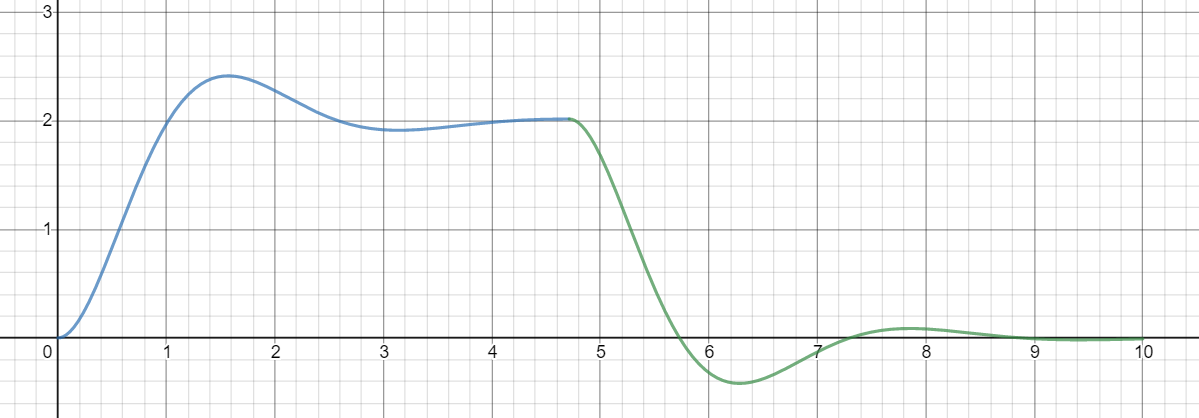
\includegraphics[scale=0.75]{nice}
\end{figure}

42.

(a) The general solution to equation (15) will be the solution to the homogeneous mass-spring system differential equation with some added terms. This is due to being able to find some linear differential operator $A_g$ that produces roots that show up as added terms in the general solution.
$$y = c_1e^{\frac{-b}{2m}}\sin(\frac{\sqrt{b^2-4mk}}{2m}) + c_2e^{\frac{-b}{2m}}\cos(\frac{\sqrt{b^2-4mk}}{2m}) + \text{ additional terms}$$

All we need to do is find roots of the quadratic the annihilator $A_{\sin(\beta t)} = \br{D^2+ \beta^2}$ makes, which are $\pm i\beta$. So tentatively the general solution is of the form:
$$c_1e^{\frac{-b}{2m}}\sin(\frac{\sqrt{b^2-4mk}}{2m}) + c_2e^{\frac{-b}{2m}}\cos(\frac{\sqrt{b^2-4mk}}{2m}) + c_3\sin(\beta t) + c_4\cos(\beta t)$$

To determine the last two coefficients we need to put the above into the original differential equation:
$$\br{mD^2 + bD + k}\sbr{c_1e^{\frac{-b}{2m}}\sin(\frac{\sqrt{b^2-4mk}}{2m}) + c_2e^{\frac{-b}{2m}}\cos(\frac{\sqrt{b^2-4mk}}{2m}) + c_3\sin(\beta t) + c_4\cos(\beta t)} = \sin(\beta t)$$
$$\to m\br{-c_3\beta^2\sin(\beta t) - c_4\beta^2\cos(\beta t)} + b\br{c_3\beta\cos(\beta t) - c_4\beta\sin(\beta t)} + k\br{c_3\sin(\beta t) + c_4\cos(\beta t)} = \sin(\beta t)$$
$$\to ... \text{ more algebra}$$

In any case these coefficients are gonna be constants that depend on the value of the other constants that appear in the system.

(b) Take an informal limit as $t$ tends to $+\infty$ to notice that the terms $$c_1e^{\frac{-b}{2m}}\sin(\frac{\sqrt{b^2-4mk}}{2m}) + c_2e^{\frac{-b}{2m}}\cos(\frac{\sqrt{b^2-4mk}}{2m})$$
vanish while the other two remain (they continue to oscillate). So the long term behavior approaches undamped sinusoidal motion given by the other two terms. \\

Section 6.3 \\

11. Find the linear differential operator $A_{x^4-x^2+11}$ that annihilates $x^4-x^2+11$.

Four derivatives will return $4!$, so one more will nullify it. $$A_{x^4-x^2+11} = D^5$$\\

17. Find the linear differential operator $A_{x^2e^{-x}\sin(2x)}$ that annihilates $x^2e^{-x}\sin(2x)$.

It was shown earlier in the section that the linear differential operator $\sbr{\br{D-\alpha}^2+\beta^2}^m$ annihilates terms of the form $x^ke^{\alpha x}\cos(\beta x)$ or $x^ke^{\alpha x}\sin(\beta x)$ for $m = k+1$. Comparing that form to $x^2e^{-x}\sin(2x)$, it is apparent that we set $k = 3$, $\alpha = -1$, and $\beta = 2$. Thus
$$A_{x^2e^{-x}\sin(2x)} = \sbr{\br{D+1}^2+4}^3$$

\end{document}